\documentclass{report}
\setlength{\parindent}{0pt} % no indentation (globally)
\usepackage{amsmath} % for math environments like align
\usepackage{cancel}  % for cancelling terms
\usepackage{graphicx} % for figures
\usepackage{caption} % for captions
\usepackage{tikz-feynman} % for Feynman diagrams

\title{NNLO (differential) predictions for Triboson processes in Soft-Approximation}
\author{Paolo Garbarino}
\date{\today}

\begin{document}

\maketitle

\section*{Introduction}
In these notes I report what has been done during my first project, namely the study of the performance of the Soft-Approximation applied to vector boson + photon (Diboson) and vector boson pair + photon (Triboson).
We first discuss why these processes are important and then we move to our method. We will first compare our predictions with the Diboson processes, for which the exact amplitudes up to NNLO are available since several years.
The possibility to directly test against exact results allows us to select a best prediction to be applied to the Tribosons as well, accompained by a suitable error estimation.

\chapter{Motivations}

\chapter{Dibosons}
This first part of the notes is based on the work done by Elvira during her semester project, focused one NLO and NNLO predictions for $W\gamma$ and $Z\gamma$. The idea is to exploit the soft-photon approximation to make predictions for both the inclusive rate and differential distributions that we can test against the exact results, available for the class of Diboson processes.
If we let the photon being soft and carry on our computation as it is, we will find already a good agreement between the soft-approximated (SA in the rest of the notes) predictions and the NNLO exact results. However, these predictions are supposed to work quite well, in principle, only when the phase-space configuration is such that the photon is really soft, i.e. it has small
energy compared to the typical scale of our process. This is the reason which led to try to consider an extension of the validity range of this kind of approximations by means of so-called 'reweighting factors' to be applied to the SA amplitude, as estensively explained later on.

\section{Theoretical Framework: Soft-Photon Approximation}
We know that the emission of a photon from the initial or final states leads to an infrared divergence when the momentum of the photon, let's label it $k$, approaches zero. In this limit, it can be shown [Peskin, Schroeder] that the exact amplitude can be written as the same amplitude without the photon times the so-called Soft-Factor (SF), the latter depending on the momenta
and electric charges of the particle emitting it. What is needed, then, is a proper projection from the set of momenta for the full amplitude to that of the reduce one (projected kinemtics), whose realization is completely arbitrary; we decided to define such a projection in a way that the invariant mass of the lepton-pair (resonance) is left unchanged, by reabsorbing the recoil 
of the 'missing' photon into the initial state (the same will hold for Tribosons).
We show how this procedure works by an explicit example (again, from Elvira's notes). 
\newpage Since the first Triboson process of interest will be $WW\gamma$, we present here the computation of the SF for $W^-\gamma$, where the LO contributing diagrams are:

% insert diagrams, TikZ
\begin{minipage}{0.3\textwidth}
    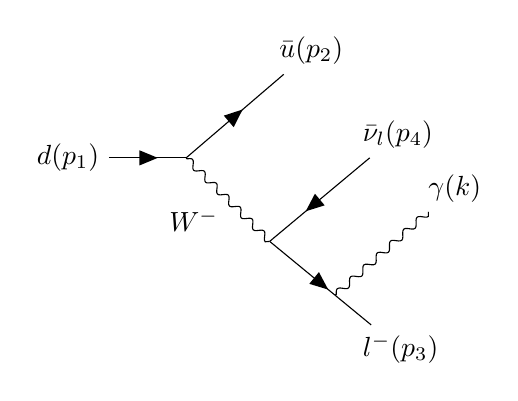
\begin{tikzpicture} % photon emitted from the FS charged lepton
    \begin{feynman}
        \vertex (a) {\(d(p_1)\)}; 
        \vertex [right=of a] (b);
        \vertex [above right=of b] (f1) {\(\bar{u}(p_2)\)};
        \vertex [below right=of b] (c);
        \vertex [above right=of c] (f2) {\(\bar{\nu}_{l}(p_4)\)};
        \vertex [below right=of c] (f3) {\(l^{-}(p_3)\)};
        \vertex at ($(c)!0.5!(f3)$) (v);  % new vertex at the midpoint of (c) and (f3)
        \vertex [above right=of v] (f4) {\(\gamma(k)\)};

        \diagram* {
            (a) -- [fermion] (b) -- [fermion] (f1),
            (b) -- [boson, edge label'=\(W^{-}\)] (c),
            (c) -- [anti fermion] (f2),
            (c) -- [fermion] (f3),
            (v) -- [boson] (f4),
        };
    \end{feynman}
\end{tikzpicture}
\end{minipage}
\hspace{3cm}
\begin{minipage}{0.3\textwidth}
    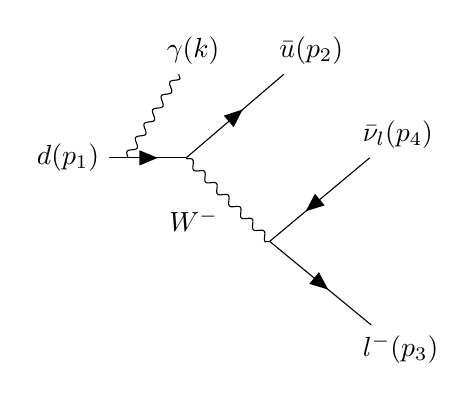
\begin{tikzpicture} % photon emitted from the IS d-quark
    \begin{feynman}
        \vertex (a) {\(d(p_1)\)}; 
        \vertex [right=of a] (b);
        \vertex [above right=of b] (f1) {\(\bar{u}(p_2)\)};
        \vertex [below right=of b] (c);
        \vertex [above right=of c] (f2) {\(\bar{\nu}_{l}(p_4)\)};
        \vertex [below right=of c] (f3) {\(l^{-}(p_3)\)};
        \vertex at ($(a)!0.5!(b)$) (v);
        \vertex [left=of f1] (f4) {\(\gamma(k)\)};

        \diagram* {
            (a) -- [fermion] (b) -- [fermion] (f1),
            (b) -- [boson, edge label'=\(W^{-}\)] (c),
            (c) -- [anti fermion] (f2),
            (c) -- [fermion] (f3),
            (v) -- [boson] (f4),
        };
    \end{feynman}
\end{tikzpicture}
\end{minipage}
\vspace{1cm}

\begin{center}
    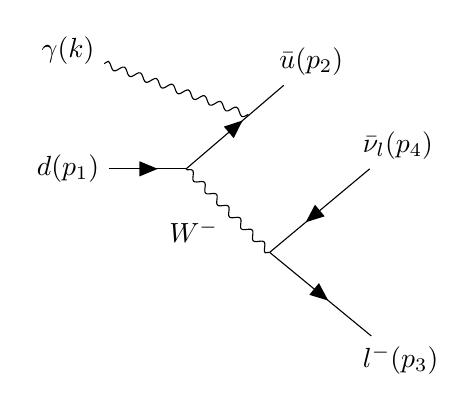
\begin{tikzpicture}[scale=0.4] % photon emitted from the IS anti u-quark
    \begin{feynman}
        \vertex (a) {\(d(p_1)\)}; 
        \vertex [right=of a] (b);
        \vertex [above right=of b] (f1) {\(\bar{u}(p_2)\)};
        \vertex [below right=of b] (c);
        \vertex [above right=of c] (f2) {\(\bar{\nu}_{l}(p_4)\)};
        \vertex [below right=of c] (f3) {\(l^{-}(p_3)\)};
        \vertex at ($(b)!0.5!(f1)$) (v);
        \vertex [above=of a] (f4) {\(\gamma(k)\)};

        \diagram* {
            (a) -- [fermion] (b) -- [fermion] (f1),
            (b) -- [boson, edge label'=\(W^{-}\)] (c),
            (c) -- [anti fermion] (f2),
            (c) -- [fermion] (f3),
            (v) -- [boson] (f4),
        };
    \end{feynman}
\end{tikzpicture}
\end{center}

The amplitude for this process reads:

\begin{align}
    M =& M_0(p_1,p_2,p_3+k,p_4)\left[i\frac{\cancel{p}_3+\cancel{k}+m_3}{(p_3+k)^2-m_3^2}\right]\left(-iQ_e\gamma^\mu\right)\epsilon_\mu^*(k) \nonumber \\
    &+ M_0(p_1-k,p_2,p_3,p_4)\left(-iQ_d\gamma^\mu\right)\epsilon_\mu^*(k)\left[i\frac{\cancel{p}_1-\cancel{k}+m_1}{(p_1-k)^2-m_1^2}\right] \nonumber \\
    &+ M_0(p_1,p_2+k,p_3,p_4)\left[i\frac{\cancel{p}_2+\cancel{k}+m_2}{(p_2+k)^2-m_2^2}\right]\left(-iQ_u\gamma^\mu\right)\epsilon_\mu^*(k)
\end{align}


where $M_0$ is the LO amplitude for the same process without the soft photon, therefore with a different set of momenta. Next, we perform the actual soft-photon limit, letting $k\to 0$, where we get:

\begin{align}
    M_0(p_1,p_2,p_3,p_4) &\sim M_0(p_1-k,p_2,p_3,p_4) \nonumber \\
    &\sim M_0(p_1,p_2+k,p_3,p_4) \nonumber \\
    &\sim M_0(p_1,p_2,p_3+k,p_4) \equiv M_0 
\end{align}

and 

\begin{align}
    (p_3-k)^2-m_3^2 &= -2p_3k \\
    (p_1-k)^2-m_1^2 &= -2p_1k \\
    (p_2+k)^2-m_2^2 &= 2p_2k
\end{align}

in the massless limit. For the squared amplitude we finally get:

\begin{align}
    \left|M\right|^2 = 2M_0^2&\left[Q_eQ_d\frac{p_3\cdot p_2}{\left(p_3\cdot k\right)\left(p_2\cdot k\right)} - Q_eQ_u\frac{p_3\cdot p_1}{\left(p_3\cdot k\right)\left(p_1\cdot k\right)} + \right.\\
    &+ \left.Q_dQ_u\frac{p_2\cdot p_1}{\left(p_2\cdot k\right)\left(p_1\cdot k\right)} + \text{terms} \propto p_i^2\right]
\end{align}

and we will neglect the terms $\propto p_i^2$ since we work in the massless limit. Of course the same procedure can be applied to the other $V+\gamma$ processes, namely $W^+\gamma$, $Z(\to l^+l^-)\gamma$ and $Z(\to \nu\bar{\nu})\gamma$, in the same straightforward way.

\section{Re-weighting factors}
As briefly mentioned at the beginning of this chapter, in order to extend the validity range of our approximation we decided to add a re-weighting-factor (RW) to our SA amplitudes. The results have been obtained by taking every contribution exact (here also the $H_2$, of course)
and then comparing how our method behaves at the level of the $H_1$ and $H_2$ contributions. I recall here the definition of these two terms:

\begin{equation}
    H_1 = \frac{2\Re\{\langle M^{(0)}|M_{fin}^{(1)}\rangle\}}{\left|M^{(0)}\right|^2}, \qquad H_2 = \frac{2\Re\{\langle M^{(0)}|M_{fin}^{(2)}\rangle\}}{\left|M^{(0)}\right|^2}
\end{equation}

where $|M_{fin}^{(1), (2)}\rangle$ are the finite reminders of the 1- and 2-loop amplitude in the $q_T$-scheme; in these expressions each matrix element is the exact one, and we have to keep in mind that, at the integration level, $H_1$ and $H_2$ are both multiplied by the exact Born-squareed again.
Here is where our RW becomes important. What we observed (see the next section) is that the agreement with the bare SA is very good, generally, only at the inclusive level, while if we look into the differential distributions we see that they are not very-well reproduced by

\begin{equation}\label{basic SA}
    H_1^{SA} = \frac{2\Re\{\langle M_{SA}^{(0)}|M_{SA, fin}^{(1)}\rangle\}}{\left|M^{(0)}\right|^2}, \qquad H_2^{SA} = \frac{2\Re\{\langle M_{SA}^{(0)}|M_{SA, fin}^{(2)}\rangle\}}{\left|M^{(0)}\right|^2}
\end{equation}

The very good agreement for the total rate comes indeed from large fluctuations in the first bins of the differential distributions, where the bulk of the cross-section lies, such that the average deviation goes away.
We will refer to Eq.(\ref{basic SA}) as to the 'un-reweighted' (no-RW) result, since at the integration level we will consider exactly the soft amplitude, namely the Drell-Yan (DY) one times the SF computed as in the previous section.
What can we do to improve this situation? One can actually try several RW procedures, each of them analysed in the following:

\begin{enumerate}
    \item $H_1$: in this case, the only RW which make sense are a no-RW or a Born re-weighted (M0M0-RW) computation
    \item $H_2$: here we can try also the M1M0-RW (interference 1-loop and Born) or the M1M1-RW (with the 1-loop squared)
\end{enumerate}

Let's break through them to explain their names.

\begin{enumerate}
    \item no-RW: we know that in the end both $H_1$ and $H_2$ are multiplied by the exact Born-squared, therefore the name 'no reweighting' comes from the fact that we directly integrate the SA amplitude
    \item M0M0-RW: this procedure consists in multiplying by the ratio of the exact and the SA Born-squared:
    
    \begin{equation}
        H_{1,2} \longrightarrow H_{1,2}\times\frac{\left|M^{(0)}\right|^2}{\left|M_{SA}^{(0)}\right|^2}
    \end{equation}

    The present RW will have important consequences when we will try to estimate a proper error to be attached to our predictions, since it leads to a non-running of the 2-loop amplitude with the regularization scale (see section about error estimation).

    \item M1M0-RW: here we perform the same as for the M0M0-RW, but with the interference between 1-loop and Born:
    
    \begin{equation}
        H_2 \longrightarrow H_2\times\frac{2\Re\{\langle M^{(0)}|M_{fin}^{(1)}\rangle\}}{2\Re\{\langle M_{SA}^{(0)}|M_{SA, fin}^{(1)}\rangle\}}
    \end{equation}

    \item M1M1-RW: 

    \begin{equation}
        H_2 \longrightarrow H_2\times\frac{\left| M_{fin}^{(1)}\right|^2}{\left| M_{SA, fin}^{(1)}\right|^2}
    \end{equation}

\end{enumerate}

\section{Setup and first results}
The results presented in this first section, where any error estimation is still missing, have been obtained by using the following setup (basically the default in MATRIX):

\vspace{0.5cm}
\begin{tabular}{cccccccc}
    \hline
    $\sqrt{s}$ [GeV] & $p_T^{j} [GeV], \left|\eta\right|_j$ & $p_T^{l} [GeV], \left|\eta\right|_l$ & $p_T^\gamma [GeV], \left|\eta\right|_\gamma$ & $dR_{l,\gamma}$ & $dR_{l,j}$ & $dR_{\gamma, j}$ \\
    \hline
    13 & $\geq 30$, $\leq 4.4$ & $\geq 25$, $\leq 2.47$ & $\geq 15$, $\leq 2.37$ & $>0.7$ & $>0.3$ & $>0.3$
\end{tabular}

\vspace{3mm}
while from the PDF side, we used \textit{NNPDF30\_lo\_as\_0118} and the corresponding sets for NLO and NNLO.
In this section we present first results for NLO, $H_1$, NNLO and $H_2$ separately for some relevant distributions, including the different RW.

\subsection{Total rate}
We start from a comparison of the total rates at the $H_1$ and $H_2$ levels between the exact and approximated results

\begin{minipage}{0.45\textwidth}
    \centering
    \includegraphics[width=\textwidth]{/Users/paologarbarino/Library/CloudStorage/OneDrive-UniversitätZürichUZH/PhD/OneDrive/Main/PhD_Notes/Plots/result.runs.combined.split.M1M1.M2M0/H1/total_rate.H1.pdf}
\end{minipage}
\hfill
\begin{minipage}{0.45\textwidth}
    \centering
    \includegraphics[width=\textwidth]{/Users/paologarbarino/Library/CloudStorage/OneDrive-UniversitätZürichUZH/PhD/OneDrive/Main/PhD_Notes/Plots/result.runs.combined.split.M1M1.M2M0/H2_no_bands/total_rate.H2.pdf}
\end{minipage}

In the upper plots we have the absolute values, while on the lower ones the relative size w.r.t. the exact results (in red for $H_1$ and in blue for $H_2$). In both contributions we see how without any RW we are already very close to the exact result, while the M0M0-RW is far off; 
for the $H_2$ we also see how the M1M0-RW performs even slightly better. The reason why the no-RW results is so good at the inclusive level will be clear from the differential distributions: in general we observe quite big fluctuations around the bulk of the cross-section, such that the 
average distance from the exact becomes tiny.
\newpage At NLO and NNLO we have the following situation:

\begin{minipage}{0.45\textwidth}
    \centering
    \includegraphics[width=\textwidth]{/Users/paologarbarino/Library/CloudStorage/OneDrive-UniversitätZürichUZH/PhD/OneDrive/Main/PhD_Notes/Plots/result.runs.combined.split.M1M1.M2M0/NLO/total_rate.NLO.pdf}
\end{minipage}
\hfill
\begin{minipage}{0.45\textwidth}
    \centering
    \includegraphics[width=\textwidth]{/Users/paologarbarino/Library/CloudStorage/OneDrive-UniversitätZürichUZH/PhD/OneDrive/Main/PhD_Notes/Plots/result.runs.combined.split.M1M1.M2M0/NNLO/total_rate.NNLO.pdf}
\end{minipage}

where the pattern is the same, with the M1M1-RW performing slightly worse than the no-RW and M1M0-RW.

\subsection{$p_{T,\gamma}$}
This is for sure one of the most important distributions, since the photon plays an important role in our approximation, being the 'soft' particle:

\begin{minipage}{0.45\textwidth}
    \centering
    \includegraphics[width=\textwidth]{/Users/paologarbarino/Library/CloudStorage/OneDrive-UniversitätZürichUZH/PhD/OneDrive/Main/PhD_Notes/Plots/result.runs.combined.split.M1M1.M2M0/H1/pT_gamma.H1.pdf}
\end{minipage}
\hfill
\begin{minipage}{0.45\textwidth}
    \centering
    \includegraphics[width=\textwidth]{/Users/paologarbarino/Library/CloudStorage/OneDrive-UniversitätZürichUZH/PhD/OneDrive/Main/PhD_Notes/Plots/result.runs.combined.split.M1M1.M2M0/H2_no_bands/pT_gamma.H2.pdf}
\end{minipage}

\begin{minipage}{0.45\textwidth}
    \centering
    \includegraphics[width=\textwidth]{/Users/paologarbarino/Library/CloudStorage/OneDrive-UniversitätZürichUZH/PhD/OneDrive/Main/PhD_Notes/Plots/result.runs.combined.split.M1M1.M2M0/NLO/pT_gamma.NLO.pdf}
\end{minipage}
\hfill
\begin{minipage}{0.45\textwidth}
    \centering
    \includegraphics[width=\textwidth]{/Users/paologarbarino/Library/CloudStorage/OneDrive-UniversitätZürichUZH/PhD/OneDrive/Main/PhD_Notes/Plots/result.runs.combined.split.M1M1.M2M0/NNLO/pT_gamma.NNLO.pdf}
\end{minipage}

Even if this is not the distribution for which this effect is very evident, we can see what we already stated before: at the $H_1$ level (but also for the NLO, even if less evident) the M0M0-RW performs way better than the no-RW, but the former always understimates the exact result in the first bins,
which are more important for what concerns the total rate, while the no-RW result oscillates crossing the exact result, eventually leading to a closer inclusive rate. The same behavior is of course observed also for the $p_{T,W}$ distribution, which is exactly the same due to the $W-\gamma$ recoil at Born-level.

\end{document}